\documentclass[physics_notes.tex]{subfiles}
\begin{document}
\section{Aula 02 - 29/03/2023}
\subsection{Motivações}
\begin{itemize}
  \item Estudar a aceleração;
  \item Entender o Movimento Retilíneo Uniformemente Variado.
\end{itemize}
\subsection{Aceleração}
  Definimos previamente a velocidade média como sendo a variação de tempo dividindo o deslocamento, sendo, portanto,
uma quantidade representando a taxa de variação da posição em um intervalo de tempo. De forma análoga,
definimos a aceleração como a taxa de variação da velocidade em um intervalo de tempo, ou seja, 
  $$
    \vec{a_{m}} = \frac{\Delta \vec{v}}{\Delta t}.
  $$
  Ainda mais, se ela for positiva, a velocidade aumenta. Caso contrário, ela diminui. Ainda repetindo o processo feito
para o caso da velocidade, podemos encontrar uma aceleração instanânea como 
    $$
      a(t) = \lim_{\Delta t\to0}\biggl[\frac{v(t + \Delta t) - v(t)}{\Delta t}\biggr] = \frac{dv(t)}{dt}
    $$
  Observe também que 
    $$
      a(t) = \frac{d}{dt}\biggl(\frac{dx(t)}{dt}\biggr) = \frac{d^{2}x}{dt^{2}}.
    $$
  Utilizando a análise dimensional, é possível encontrar a dimensão da aceleração como $[a]=\frac{[v]}{[t]} = \frac{\frac{[L]}{[t]}}{[t]} = \frac{[L]}{[t]^{2}}.$ Assim,
se o sistema de medida for o Sistema Internacional, $[a] = \frac{m}{s^{2}}$.

    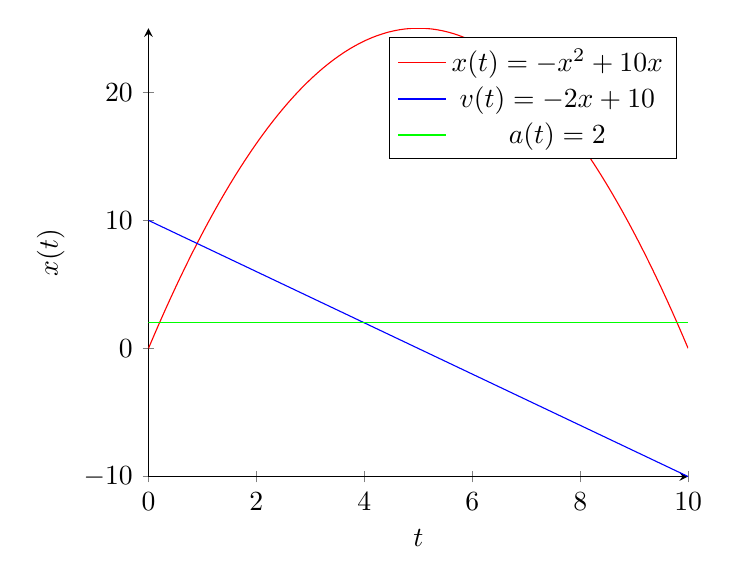
\begin{tikzpicture}
    \begin{axis}[
        axis lines = left,
        xlabel = \(t\),
        ylabel = {\(x(t)\)},
    ]
    \addplot [
        domain=0:10,
        samples=100, 
        color=red,
    ]
    {-x^2 + 10*x};
    \addlegendentry{\(x(t) = -x^{2}+10x\)}
    \addplot[
      domain=0:10,
      samples=100,
      color=blue,
    ]
    {-2*x + 10};
    \addlegendentry{\(v(t) = -2x + 10\)},
      \addplot[
        domain=0:10,
        samples=100,
        color=green,
      ]
      {2};
    \addlegendentry{\(a(t) = 2\)},
    \end{axis}
  \end{tikzpicture}

\subsection{Movimento Retilíneo Uniformemente Variado.}
  Sabendo que $a =\displaystyle \frac{d^{2}x(t)}{dt^{2}}$, podemos fazer o caminho oposto para encontrar uma fórmula para
  a posição sabendo a aceleração. De fato, dado um intervalo de tempo $[t_{0}, t],$
  $$
    v(t) = \int_{t_{0}}^{t}a(t)dt = at \biggl|_{t_{0}}^{t}\biggr. = at - at_{0}
  $$
  Sabemos, também, que $v(t) - v(t_{0}) = \Delta v$, tal que 
    $$
      v(t) = v(t_{0}) + a(t-t_{0}) = v_{0} + a(t-t_{0})
    $$
  Além disso, vimos que 
    $$
      \Delta x = x(t) - x(t_{0}) = \int_{t_{0}}^{t}v(t) dt.
    $$
  Juntando tudo, segue a fórmula dita: 
  \begin{align*}
    x(t) - x(t_{0}) &= \overbrace{\int_{t_{0}}^{t}[v_{0} + a(t-t_{0})]dt}^{\int_{}^{}f(t) + g(t)dt = \int_{}^{}f(t)dt + \int_{}^{}g(t)dt}= \overbrace{\int_{t_{0}}^{t}v_{0}dt}^{\int_{}^{}c dt = ct} + \overbrace{\int_{t_{0}}^{t}atdt}^{\int_{}^{}t^{n}dt = \frac{t^{n+1}}{n+1}} - \int_{t_{0}}^{t}at_{0}dt\\
                    & \Rightarrow x(t) - x(t_{0})  =  v_{0}t \biggl|_{t_{0}}^{t}\biggr. + a\frac{t^{2}}{2} \biggl|_{t_{0}}^{t}\biggr. - at_{0}t \biggl|_{t_{0}}^{t}\biggr. \\
                    &= v_{0}(t-t_{0}) + a \frac{(t^{2} - t_{0}^{2})}{2} - at_{0}(t-t_{0}) \\
                    &= v_{0}(t-t_{0}) + a \frac{t^{2}-t_{0}^{2}}{2} - at_{0}t + at_{0}^{2} = v_{0}t - v_{0}t_{0} + \frac{a}{2}(t^{2}-2t_{0}t + 2t_{0}^{2})\\
                    &= v_{0}(t-t_{0}) + \frac{a}{2}(t-t_{0})^{2}\\
                    & \Rightarrow x(t) = x(t_{0}) + v_{0}(t-t_{0}) + \frac{1}{2}a(t-t_{0})^{2}.
  \end{align*}
  Com isso, no caso em que $t_{0} = 0$, segue que 
   $$
    \boxed{x(t) = x_{0} + v_{0}t + \frac{at^{2}}{2}}     
   $$
  Uma coisa notável é que todas essas fórmulas estão dependentes de tempo. No entanto, será que é possível
se livrar dessa variável e relacionar, por exemplo, velocidade e posição? A resposta é sim! E vamos mostrar como a seguir,
na equação conhecida como Equação de Torricelli. Com efeito,
 \begin{align*}
   &(I)\quad (t-t_{0}) = \frac{v(t)-v_{0}}{a} = \frac{v-v_{0}}{a}\\
   &(II)\quad x(t) = x_{0} + v_{0}(t-t_{0}) + \frac{1}{2}a(t-t_{0})^{2}\\
   &(I\text{ com }II)\quad x = x_{0} + v_{0}\frac{v-v_{0}}{a} + \frac{1}{2}a \frac{v-v_{0}}{a} \\
   & \Rightarrow x = x_{0} + \frac{1}{a}\biggl\{v_{0}v - v_{0}^{2} + \frac{1}{2}(v^{2}-2vv_{0}+v_{0}^{2})\biggr\}\\
   & = x_{0} + \frac{1}{a}\biggl\{-v_{0}^{2} + \frac{v^{2}}{2} + \frac{v_{0}^{2}}{2}\biggr\}\\
   & \Rightarrow x - x_{0} = \frac{1}{2a}\biggl[v^{2}-v_{0}^{2}\biggr] \Longleftrightarrow [v^{2} - v_{0}^{2}] = 2a(x-x_{0}).
 \end{align*}
 Portanto, chegamos na Equação de Torricelli
  $$
  \boxed{v^{2} = v_{0}^{2} + 2a(x-x_{0})}
  $$
  Para reforçar o que foi visto até agora, vejamos um exemplo.
 \begin{example}
   Suponha que um carro freia uniformemente, passando de 60km/h para 30km/h em 5 segundos. Qual é a distância
que o carro percorrerá até parar? Em quanto tempo?

  \textbf{Solução}: Sabemos que $x(t) = x_{0} + v_{0}(t-t_{0}) + \frac{1}{2}a(t-t_{0})^{2}, v(t) = v_{0} + a(t-t_{0}),
\text{ e }v^{2} = v_{0}^{2} + 2a(x-x_{0}).$ Além disso, como é até o carro parar, a velocidade final é 0km/h, a variação
de tempo até o momento em que a velocidade atinge 30km/h (=8.333m/s) é dada como $\Delta t = 5 - 0 = 5$s , sendo a velocidade inicial 60km/h (=16,666m/s). 
Pela equação dois, 
  $$
    a = \frac{v(t_{1}) - v_{0}}{t_{1}-t_{0}} = \frac{8.33 - 16.66}{5} = -1.66\frac{m}{s^{2}}
  $$
  Agora, para obter a distância, sendo $v_{2} = 0km/h$ o valor da aceleração no tempo em que o carro para (o segundo percurso),
utilizamos Torricelli para obter o deslocamento no pedaço final do percurso
  $$
    v_{2}^{2} = v_{1}^{2} + 2a(x_{2}-x_{1}) \Rightarrow 0 = 8.33^{2} + 2(-1.66)\Delta x_{2}
  $$
  Assim, isolando o $\Delta x_{2},$  
    $$
    \Delta x_{2} = \frac{8.33^{2}}{3.32} = \text{ Professora vai passar na próxima aula.}
    $$
  Ademais, para encontrar todo o caminho que o carro andou, temos 
    $$
      0 = v_{0}^{2} + 2a(x_{2} - x_{0}) = 16.66^{2} + 2(-1.66)\Delta x \Rightarrow \Delta x = \frac{16.66^{2}}{3.32}
    $$
  Finalmente, o instante de tempo pode ser encontrado fazendo 
    $$
    v_{2}(t) = v_{1} + a(t_{2}-t_{0}) \Rightarrow 0 = 8.33 - 1.66\Delta t_{2} \Rightarrow \Delta t_{2} = 5s.\text{ \qedsymbol}
    $$
 \end{example}

\end{document}
